\documentclass[final]{beamer}
\usepackage[orientation=portrait,size=a0,scale=1.2]{beamerposter}

% ---------- Paquetes seguros ----------
\usepackage[utf8]{inputenc}
\usepackage[T1]{fontenc}
\usepackage{lmodern}
\usepackage{graphicx}
\usepackage{amsmath, amssymb, bm}
\usepackage{booktabs}
\usepackage{qrcode}
\usepackage{tikz}
\usetikzlibrary{arrows.meta, positioning, shapes.geometric}

% ---------- Colores suaves ----------
\definecolor{primary}{RGB}{25,118,210}
\definecolor{accent}{RGB}{5,150,105}

\setbeamercolor{block title}{fg=white,bg=primary}
\setbeamercolor{block body}{fg=black,bg=white}
\setbeamercolor{normal text}{fg=black,bg=white}

\begin{document}
\begin{frame}[t]

\begin{columns}[t,totalwidth=\textwidth]
  \begin{column}{0.1\textwidth}
    \centering
    
\includegraphics[width=0.9\linewidth]{logo_unison.png}
  \end{column}

  \begin{column}{0.9\textwidth}
    \centering
    {\bfseries\Huge Explorando sistemas cuánticos con Python: una guía para el salón de clases\par}
    \vspace{1em}
    {\Large Rafael Obed Egurrola Corella \quad (Asesor: Dr.\ Adrián Duarte)\par}
    \vspace{0.5em}
    {\large Universidad de Sonora\par}
    \vspace{0.5em}
    {\large Congreso Nacional de Física, 2025\par}
  \end{column}

\end{columns}

  
\begin{columns}[t,totalwidth=\textwidth]

% ===========================================================
% COLUMNA 1 — INTRO + NUMEROV
% ===========================================================
\begin{column}{0.32\textwidth}

% ----- INTRODUCCIÓN -----
\begin{block}{Introducción y motivación}
\begin{itemize}
  \item La física contemporánea se apoya fuertemente en la computación.
  \item Integramos \textbf{implementaciones numéricas en Python} directamente en los cursos de mecánica cuántica.
  \item Dos niveles:
  \begin{enumerate}
    \item \textbf{Numerov}: oscilador armónico 1D y radial de H.
    \item \textbf{Hartree--Fock (RHF)}: diatómicos sencillos (H$_2$, HeH$^+$).
  \end{enumerate}
  \item Objetivo docente: avanzar de \emph{comprender/aplicar} a \emph{analizar/evaluar/crear}.
\end{itemize}
\end{block}

% ----- NUMEROV: teoría + imágenes -----
\begin{block}{Método de Numerov (1D)}
\textbf{Ecuación de Schrödinger 1D:}
\[
  -\frac{\hbar^2}{2m}\,\psi''(x) + V(x)\,\psi(x) = E\,\psi(x).
\]
Si $\psi''(x)=f(x)\,\psi(x)$, el esquema de \textbf{Numerov} (paso $h$) es
\[
  \psi_{n+1} =
  \frac{2\!\left(1-\tfrac{5}{12}h^2 f_n\right)\psi_n -
        \left(1+\tfrac{1}{12}h^2 f_{n-1}\right)\psi_{n-1}}
       {1+\tfrac{1}{12}h^2 f_{n+1}}.
\]
\textbf{Notas didácticas breves:}
\begin{itemize}
  \item Precisión de orden 6, estable para potenciales suaves.
  \item Discretización de frontera y búsqueda de $E$ por \emph{shooting} / nodos.
  \item Comparación con soluciones analíticas para OA y H.
\end{itemize}

\begin{center}
  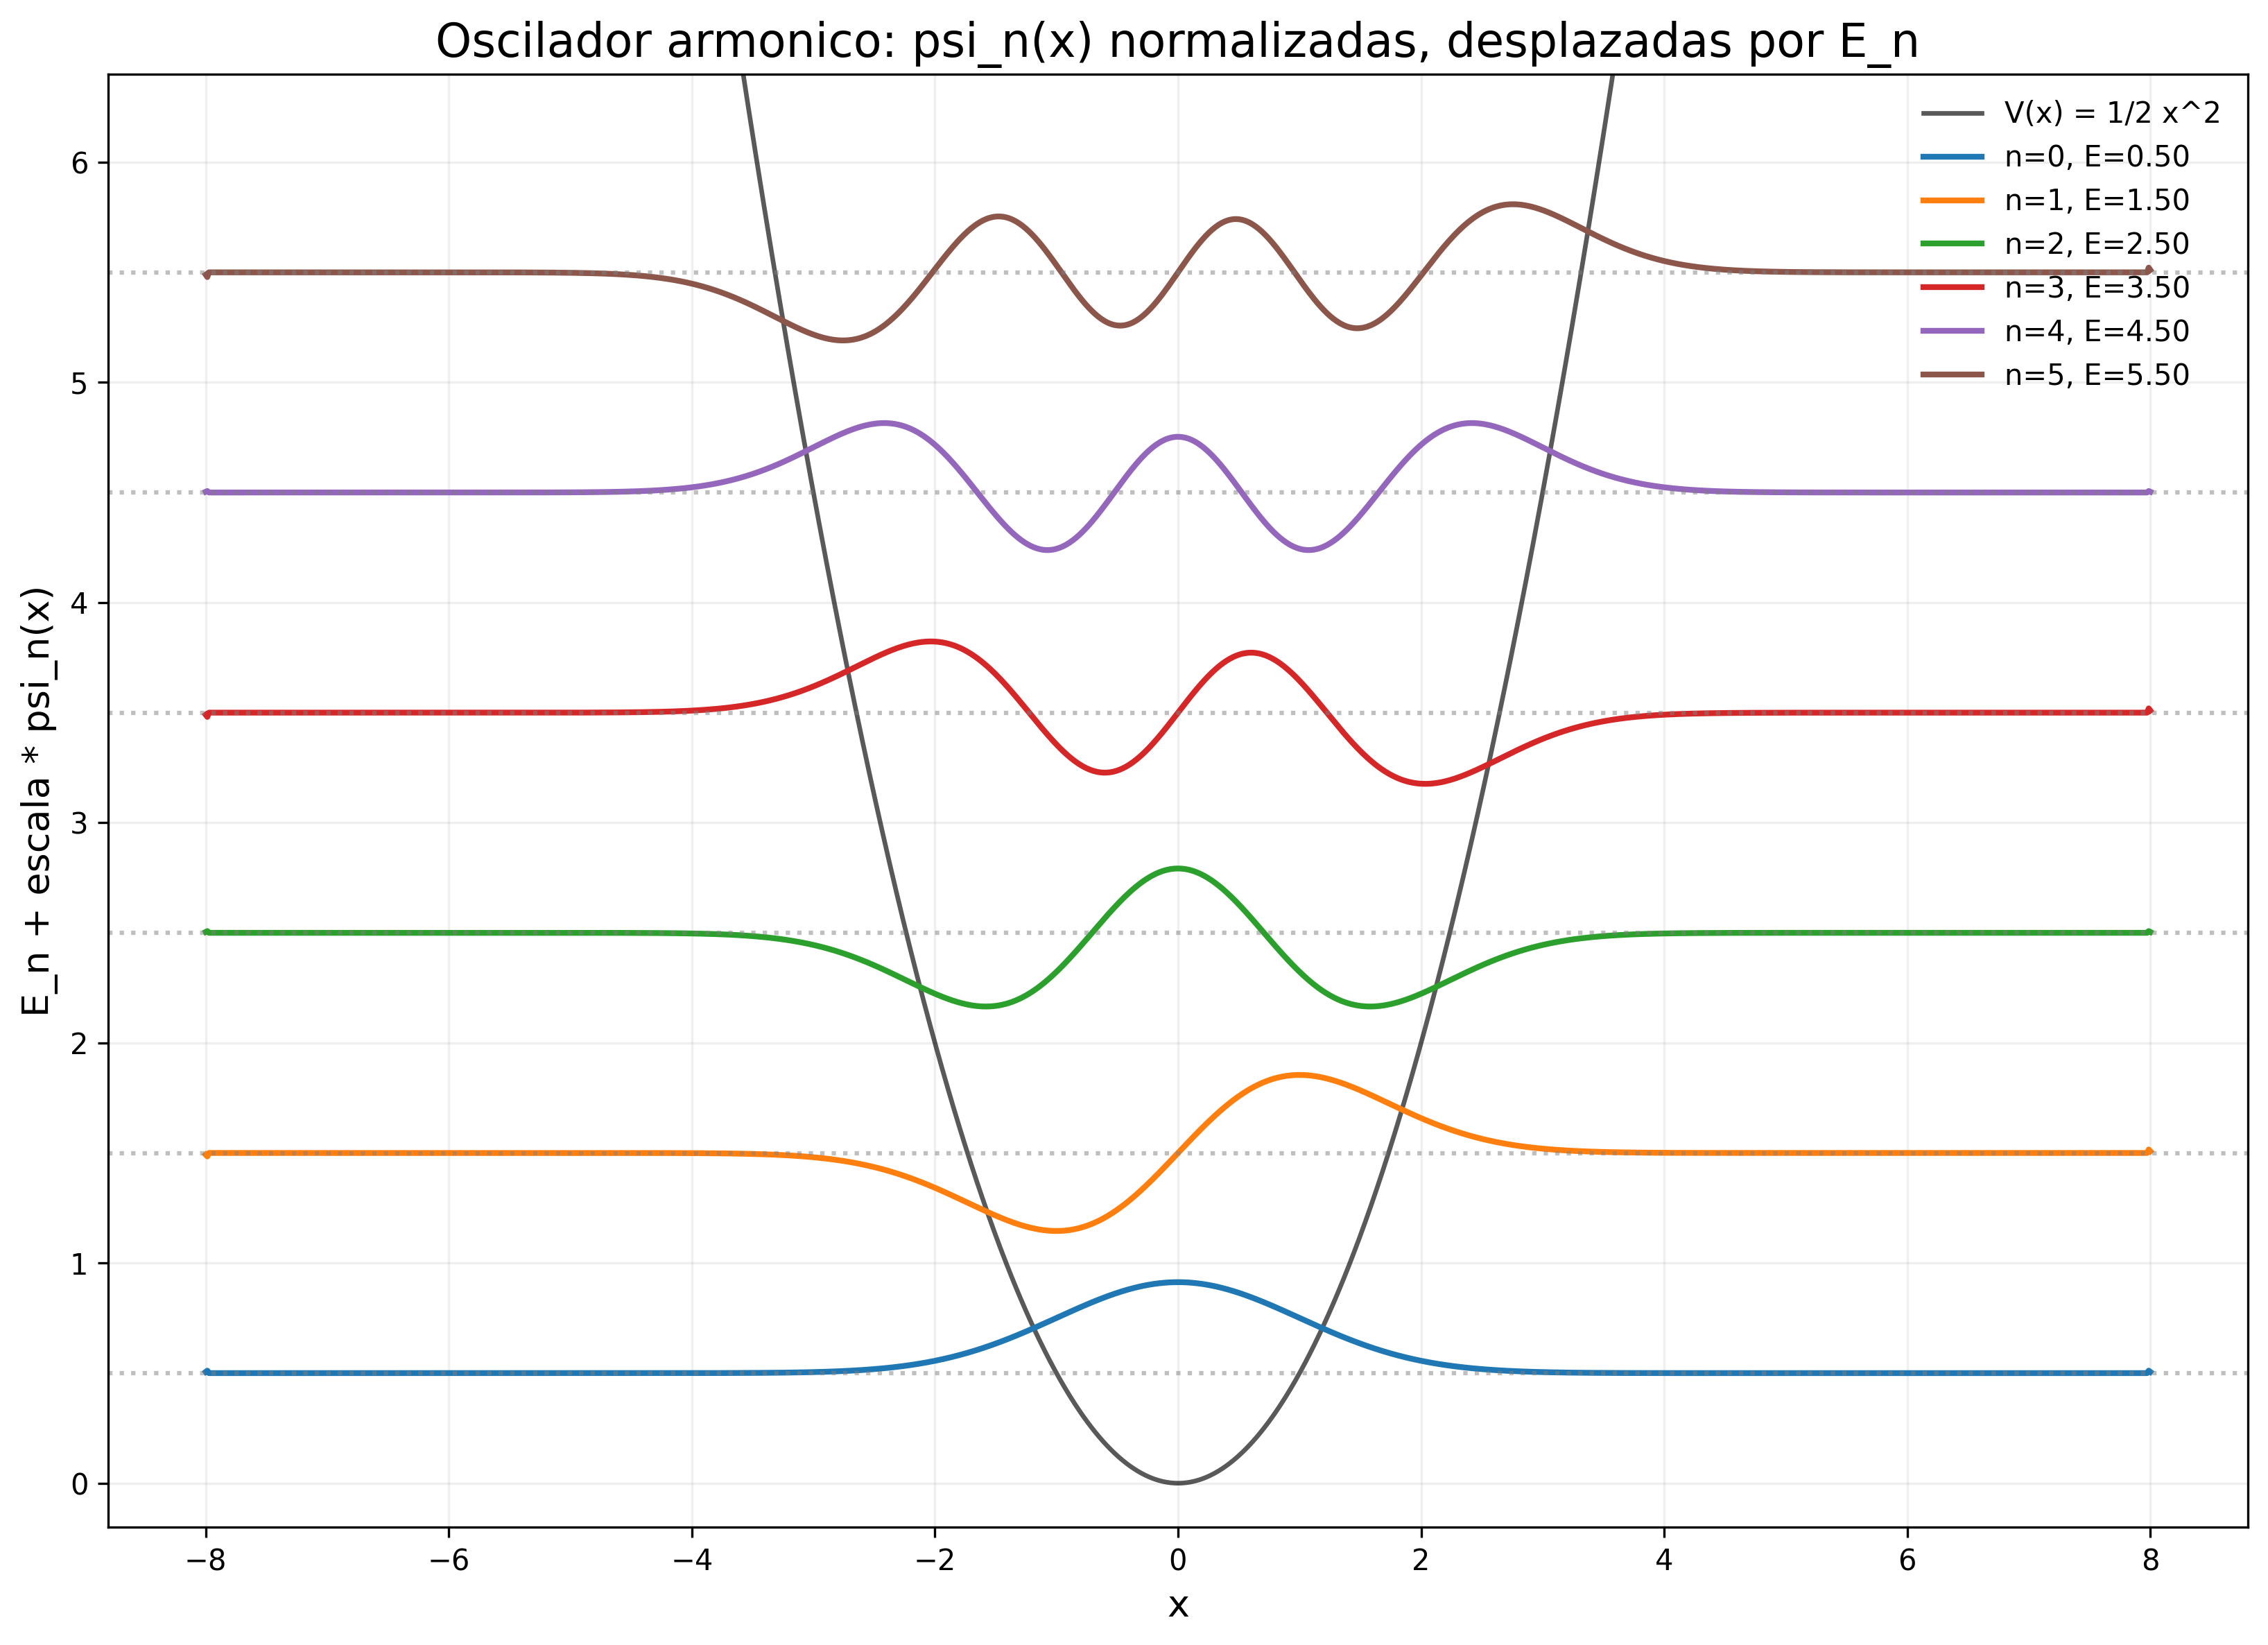
\includegraphics[width=\linewidth]{harmonic.png}\\[-0.2em]
  {\small Estados del oscilador armónico (Numerov).}\\[0.6em]
  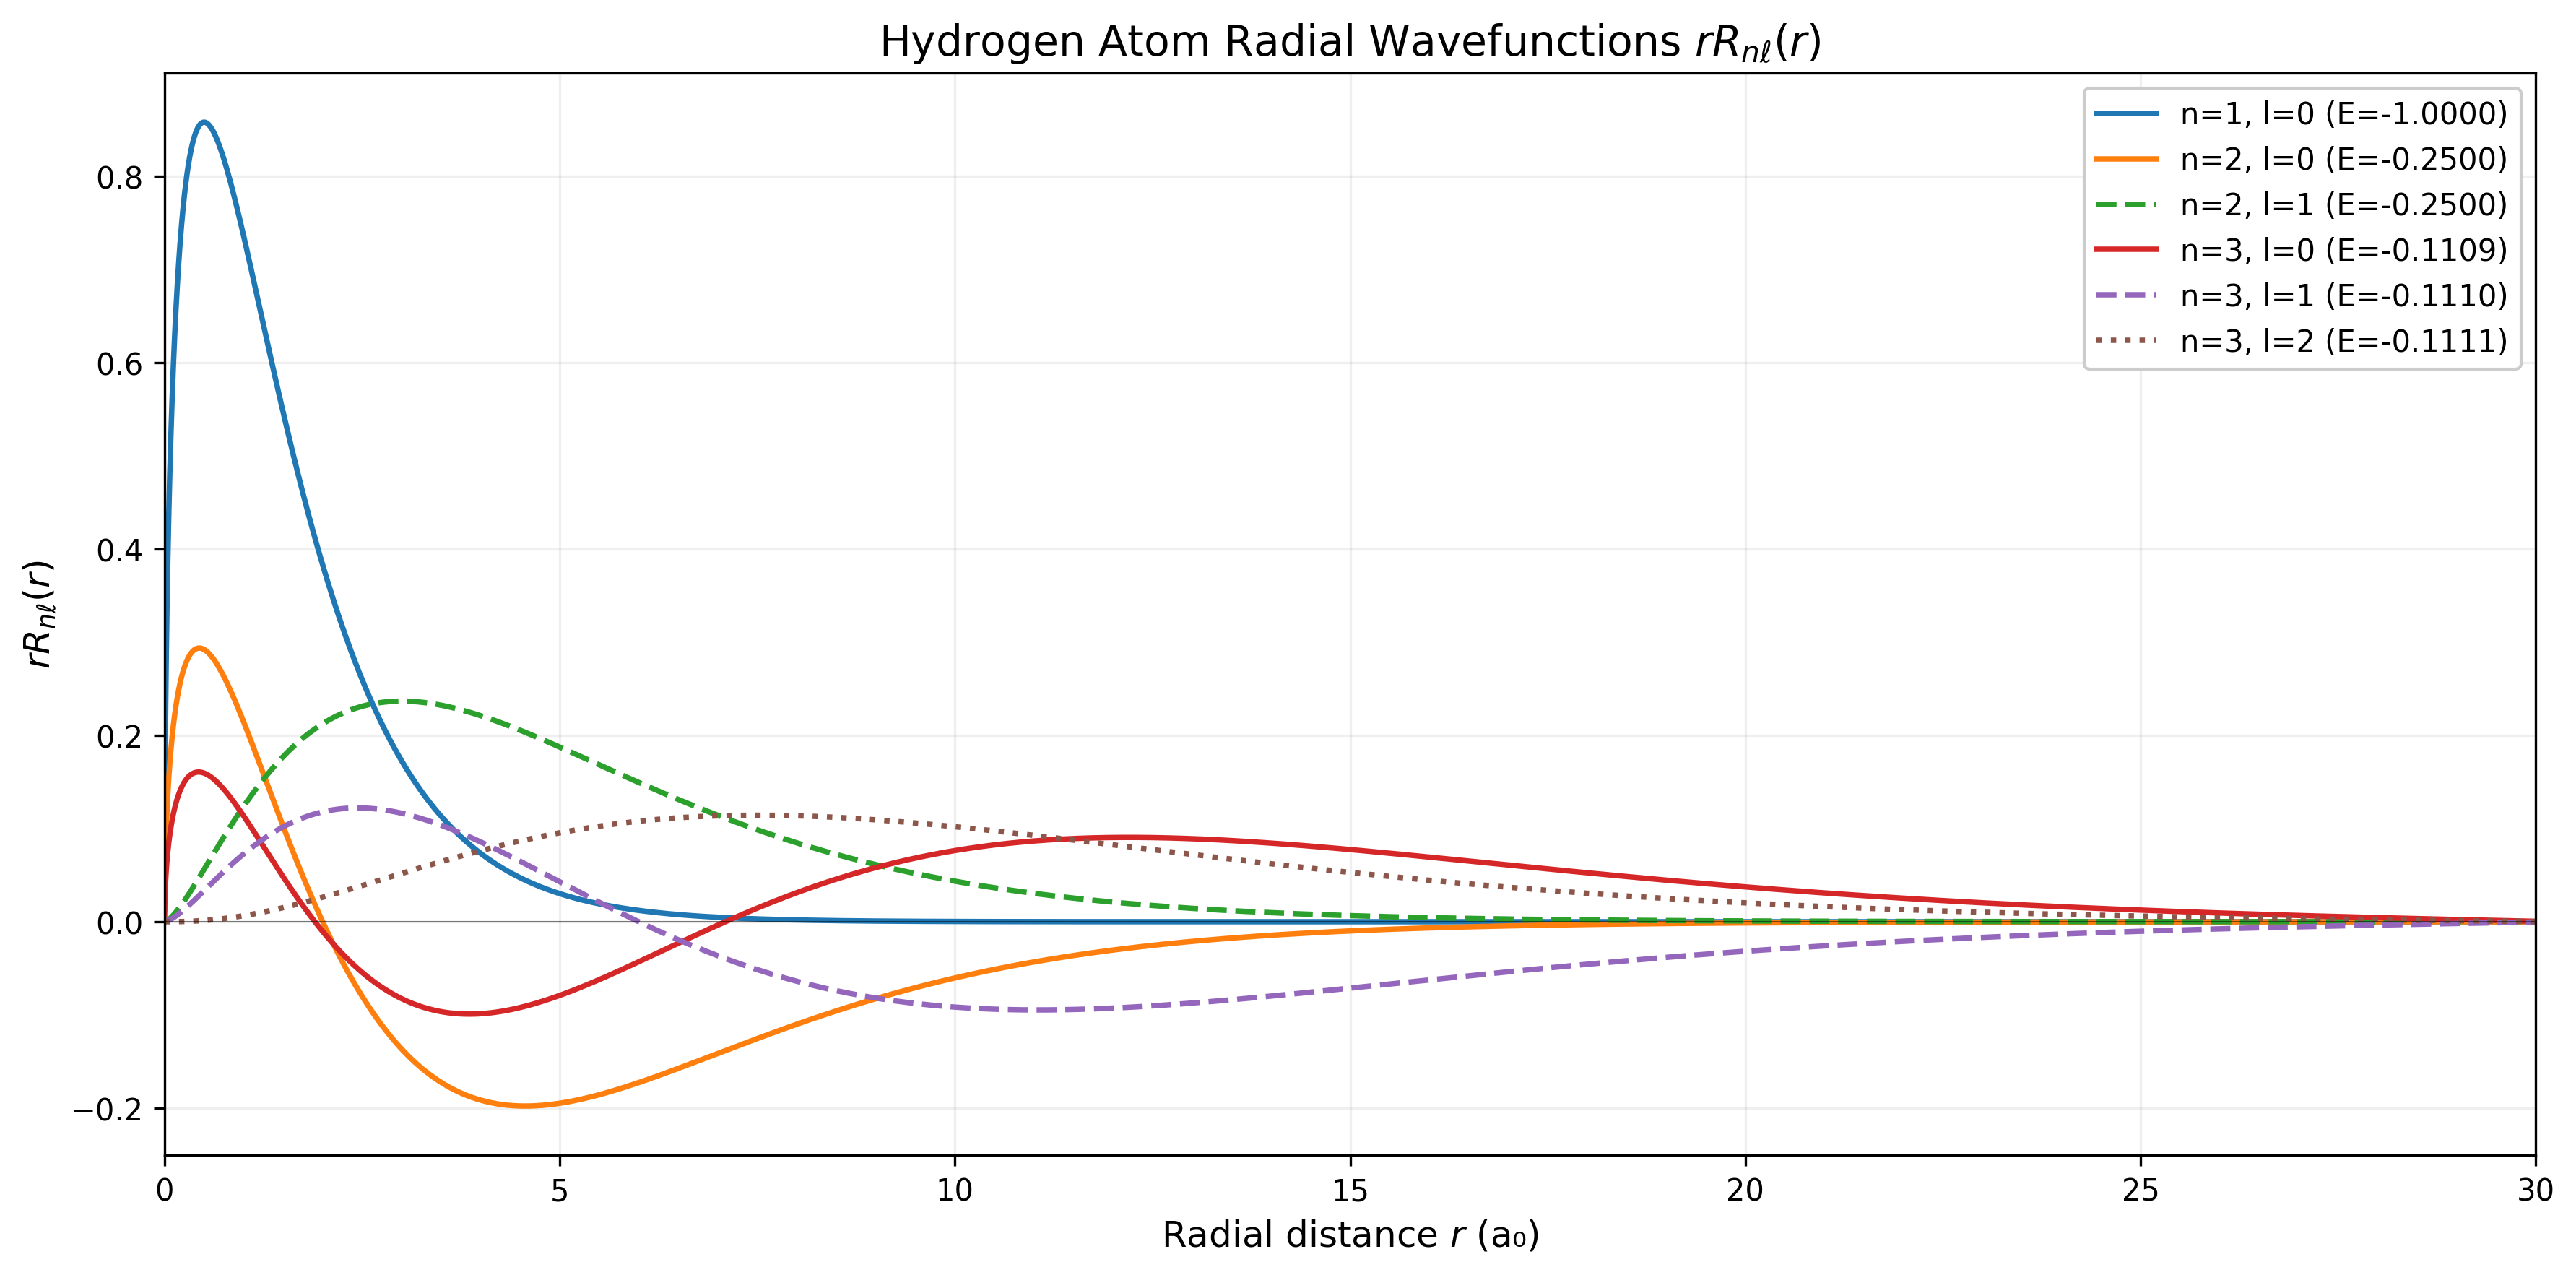
\includegraphics[width=\linewidth]{hydrogen.png}\\[-0.2em]
  {\small Funciones radiales del hidrógeno (Numerov).}
\end{center}


% \begin{columns}
%   \begin{column}{0.5\textwidth}
%     \begin{center}
%       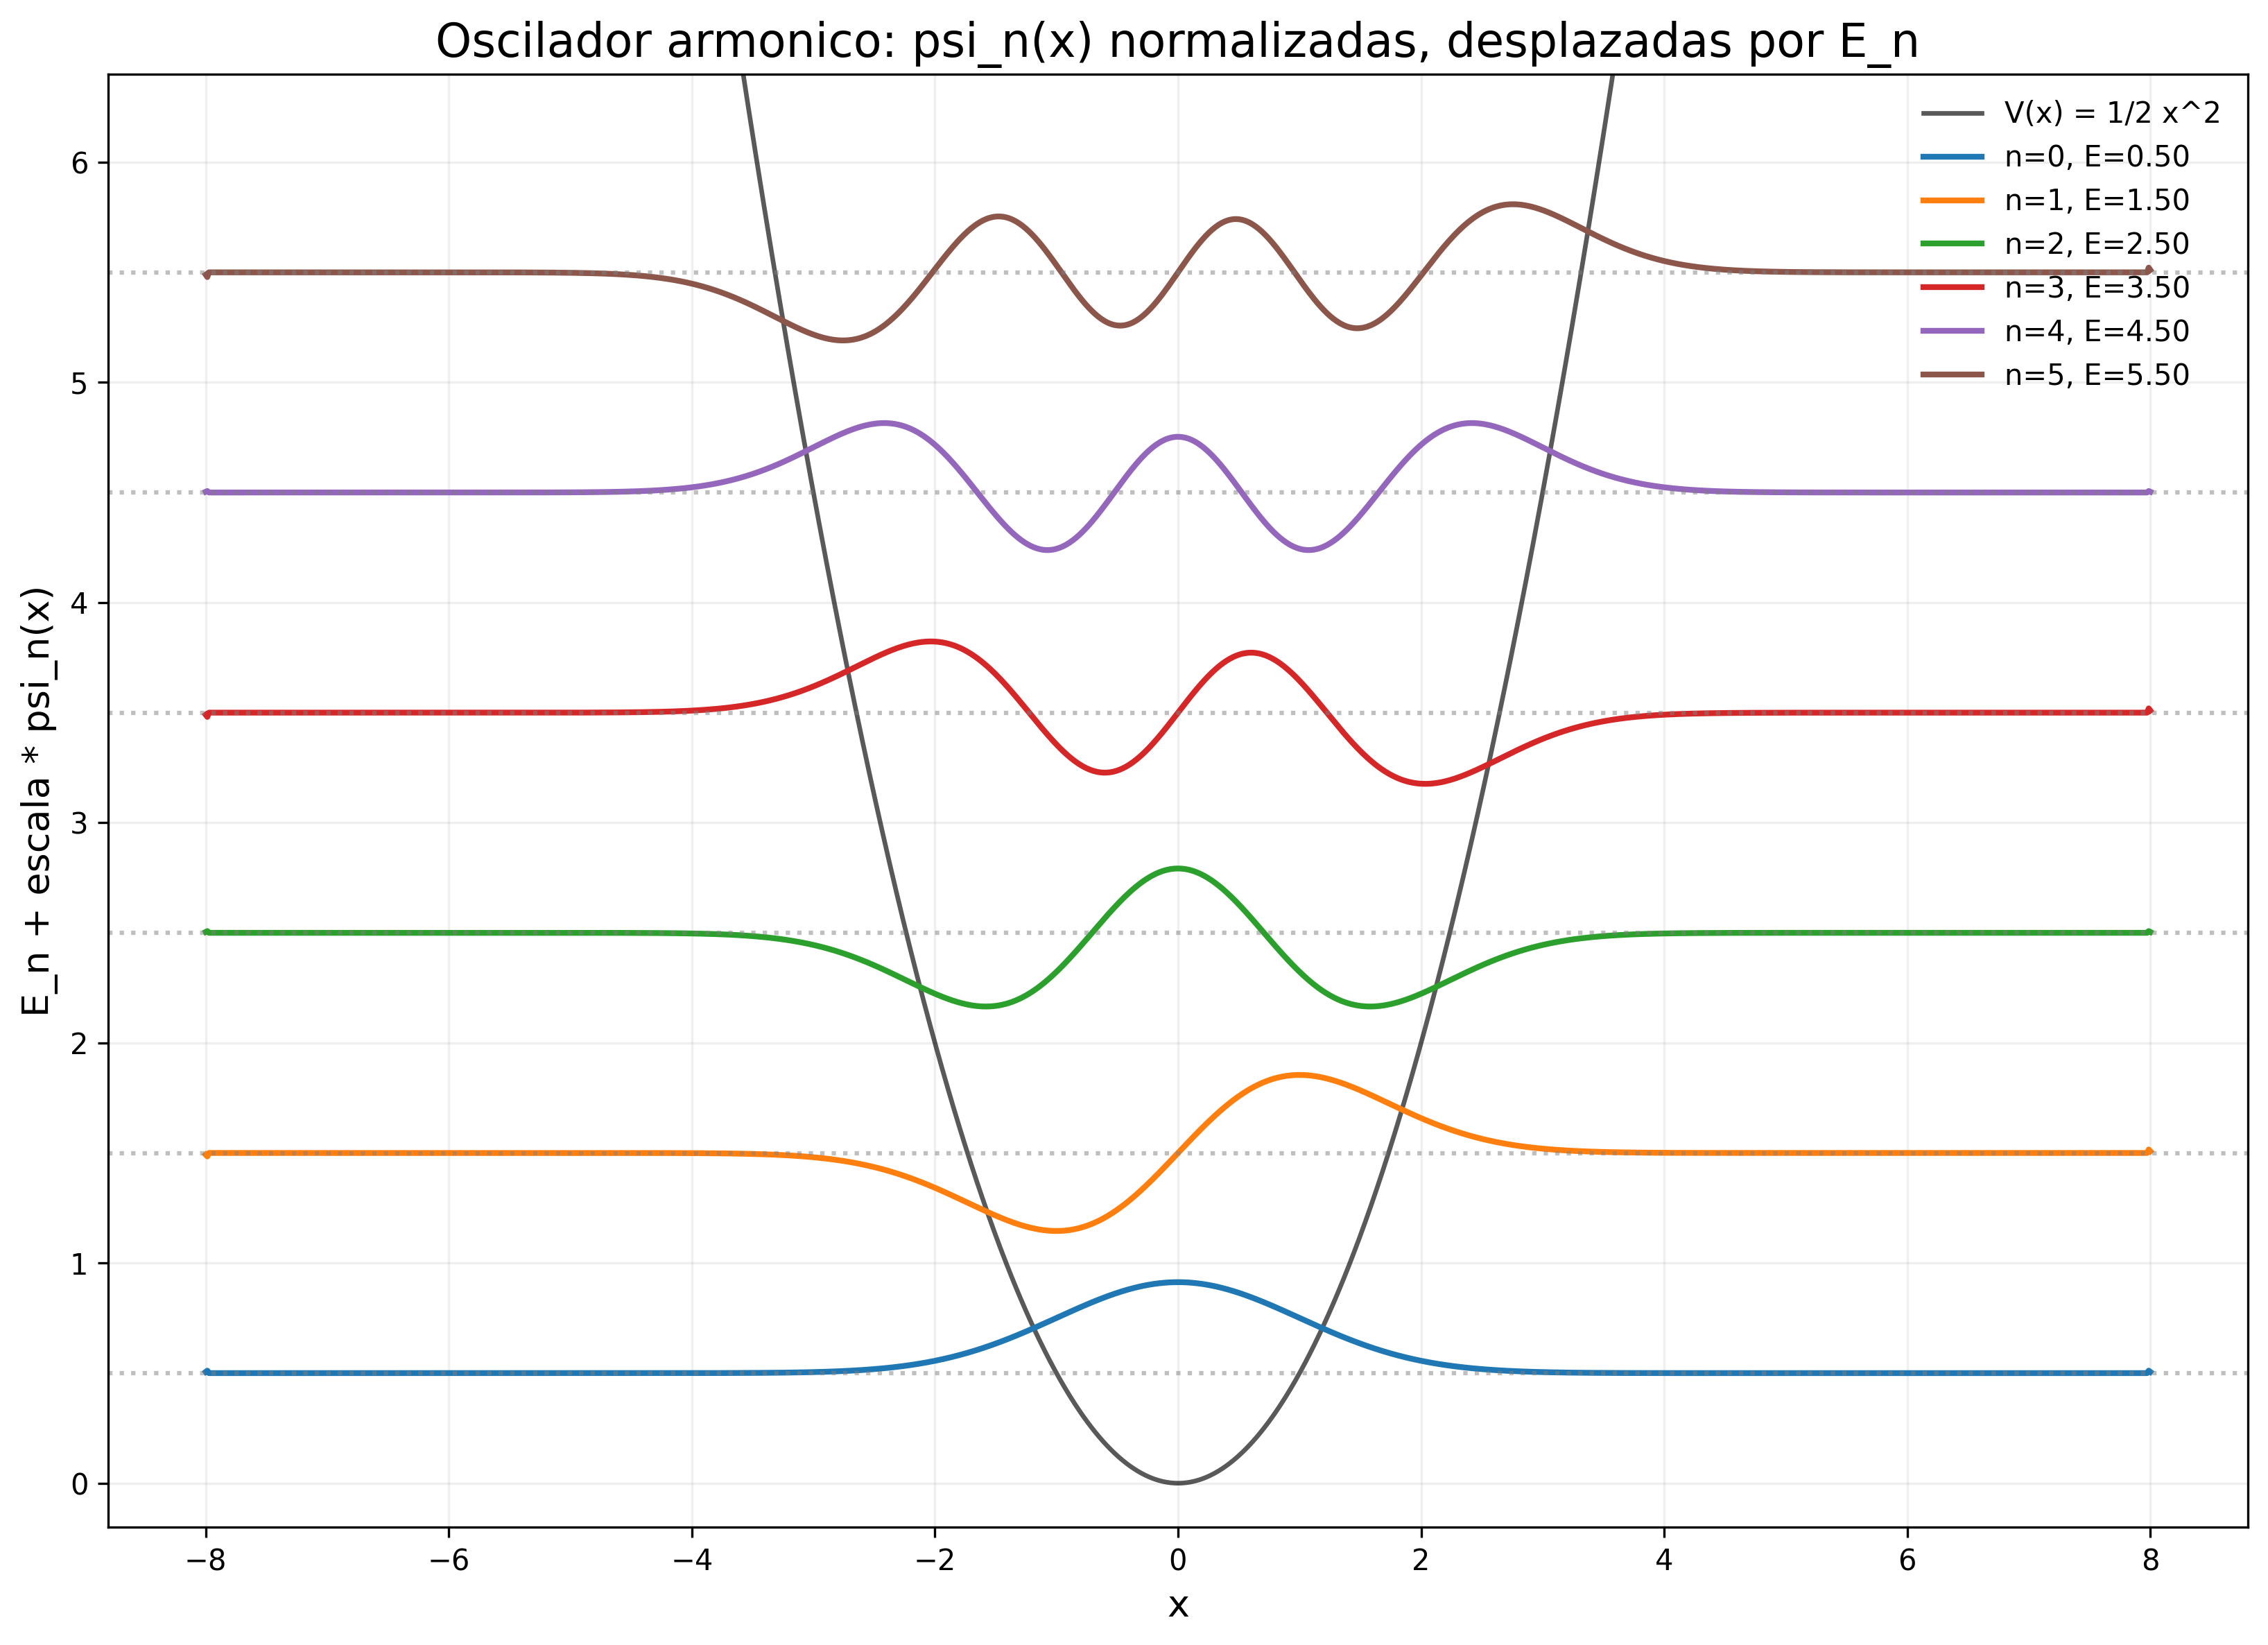
\includegraphics[width=\linewidth]{harmonic.png}\\[-0.2em]
%       {\small Estados del oscilador armónico (Numerov).}\\[0.6em]
%     \end{center}
%   \end{column}

%   \begin{column}{0.5\textwidth}
%     \begin{center}
%     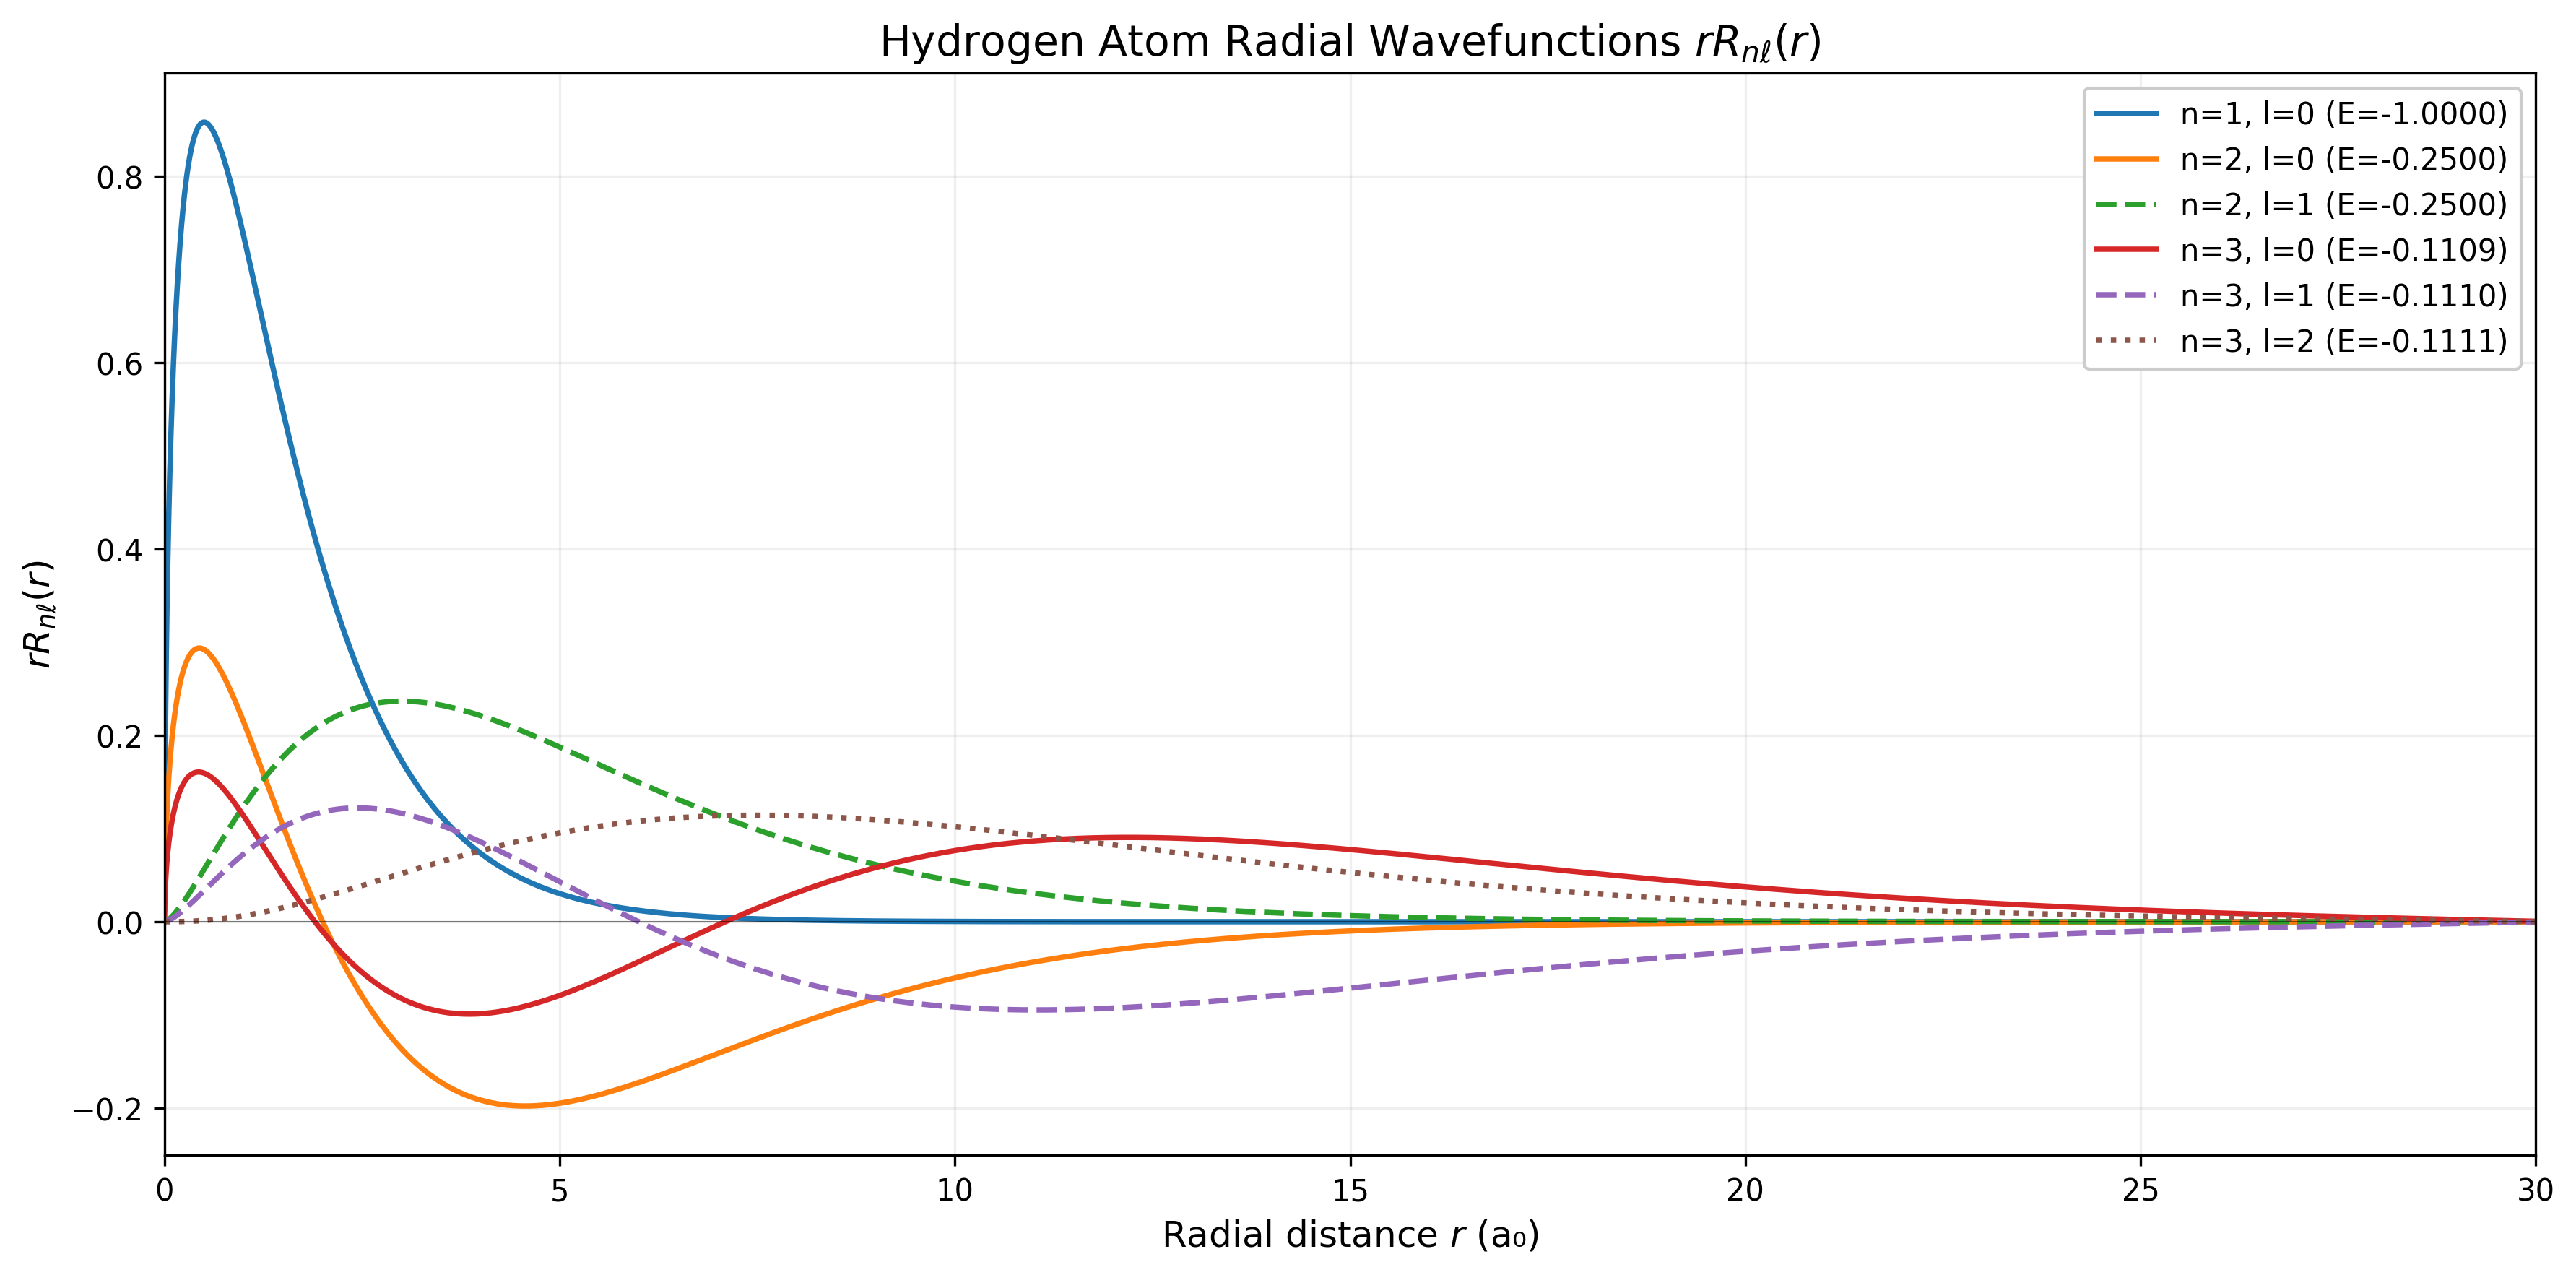
\includegraphics[width=\linewidth]{hydrogen.png}\\[-0.2em]
%     {\small Funciones radiales del hidrógeno (Numerov).}
%     \end{center}
%   \end{column}
% \end{columns}

\end{block}

\end{column}

% ===========================================================
% COLUMNA 2 — HARTREE–FOCK (RHF) COMPLETO
% ===========================================================
\begin{column}{0.36\textwidth}

\begin{block}{Hartree--Fock (RHF): Formulación y SCF}
\textbf{Ecuaciones de Roothaan--Hall:}
\[
  \mathbf{F}\,\mathbf{C} = \mathbf{S}\,\mathbf{C}\,\boldsymbol{\varepsilon},
\]
donde $\mathbf{F}$ es el operador de Fock, $\mathbf{S}$ la matriz de traslape, $\mathbf{C}$ coeficientes de los orbitales moleculares y $\boldsymbol{\varepsilon}$ energías orbitales (teorema de Koopmaans).

\[F_{\mu\nu} = H^{\mathrm{core}}_{\mu\nu} + \sum_{\lambda\sigma} P_{\lambda\sigma} \Big[(\mu\nu|\lambda\sigma) - \tfrac12\,(\mu\sigma|\lambda\nu)\Big], \]
\[P_{\mu\nu} &= 2 \sum_a^{N/2} C_{\mu a}C_{\nu a}^{*} \]
  

\medskip
\textbf{Ciclo SCF (esquema):}
\begin{center}
\begin{tikzpicture}[
  node distance=1.6cm, every node/.style={align=center},
  box/.style={rounded corners, draw=primary, very thick, fill=white, inner sep=6pt},
  >={Stealth[length=6pt]}
]
\node[box] (int) {Integrales \\ $S,\,T,\,V,\,$ERIs};
\node[box, below=of int] (fock) {Construir $\mathbf{F}[\mathbf{P}]$};
\node[box, below=of fock] (diag) {Diagonalizar \\ $\mathbf{F'}\mathbf{C'}=\mathbf{C'}\varepsilon$};
\node[box, below=of diag] (dens) {Actualizar $\mathbf{P}=2\,\mathbf{C}_{\text{occ}}\mathbf{C}_{\text{occ}}^\top$};
\draw[->,thick] (int) -- (fock);
\draw[->,thick] (fock) -- (diag);
\draw[->,thick] (diag) -- (dens);
\draw[->,thick] (dens) to[bend right=50] node[right]{\small hasta converger} (fock);
\end{tikzpicture}
\end{center}
\end{block}

\begin{block}{Resultados RHF}
\begin{center}
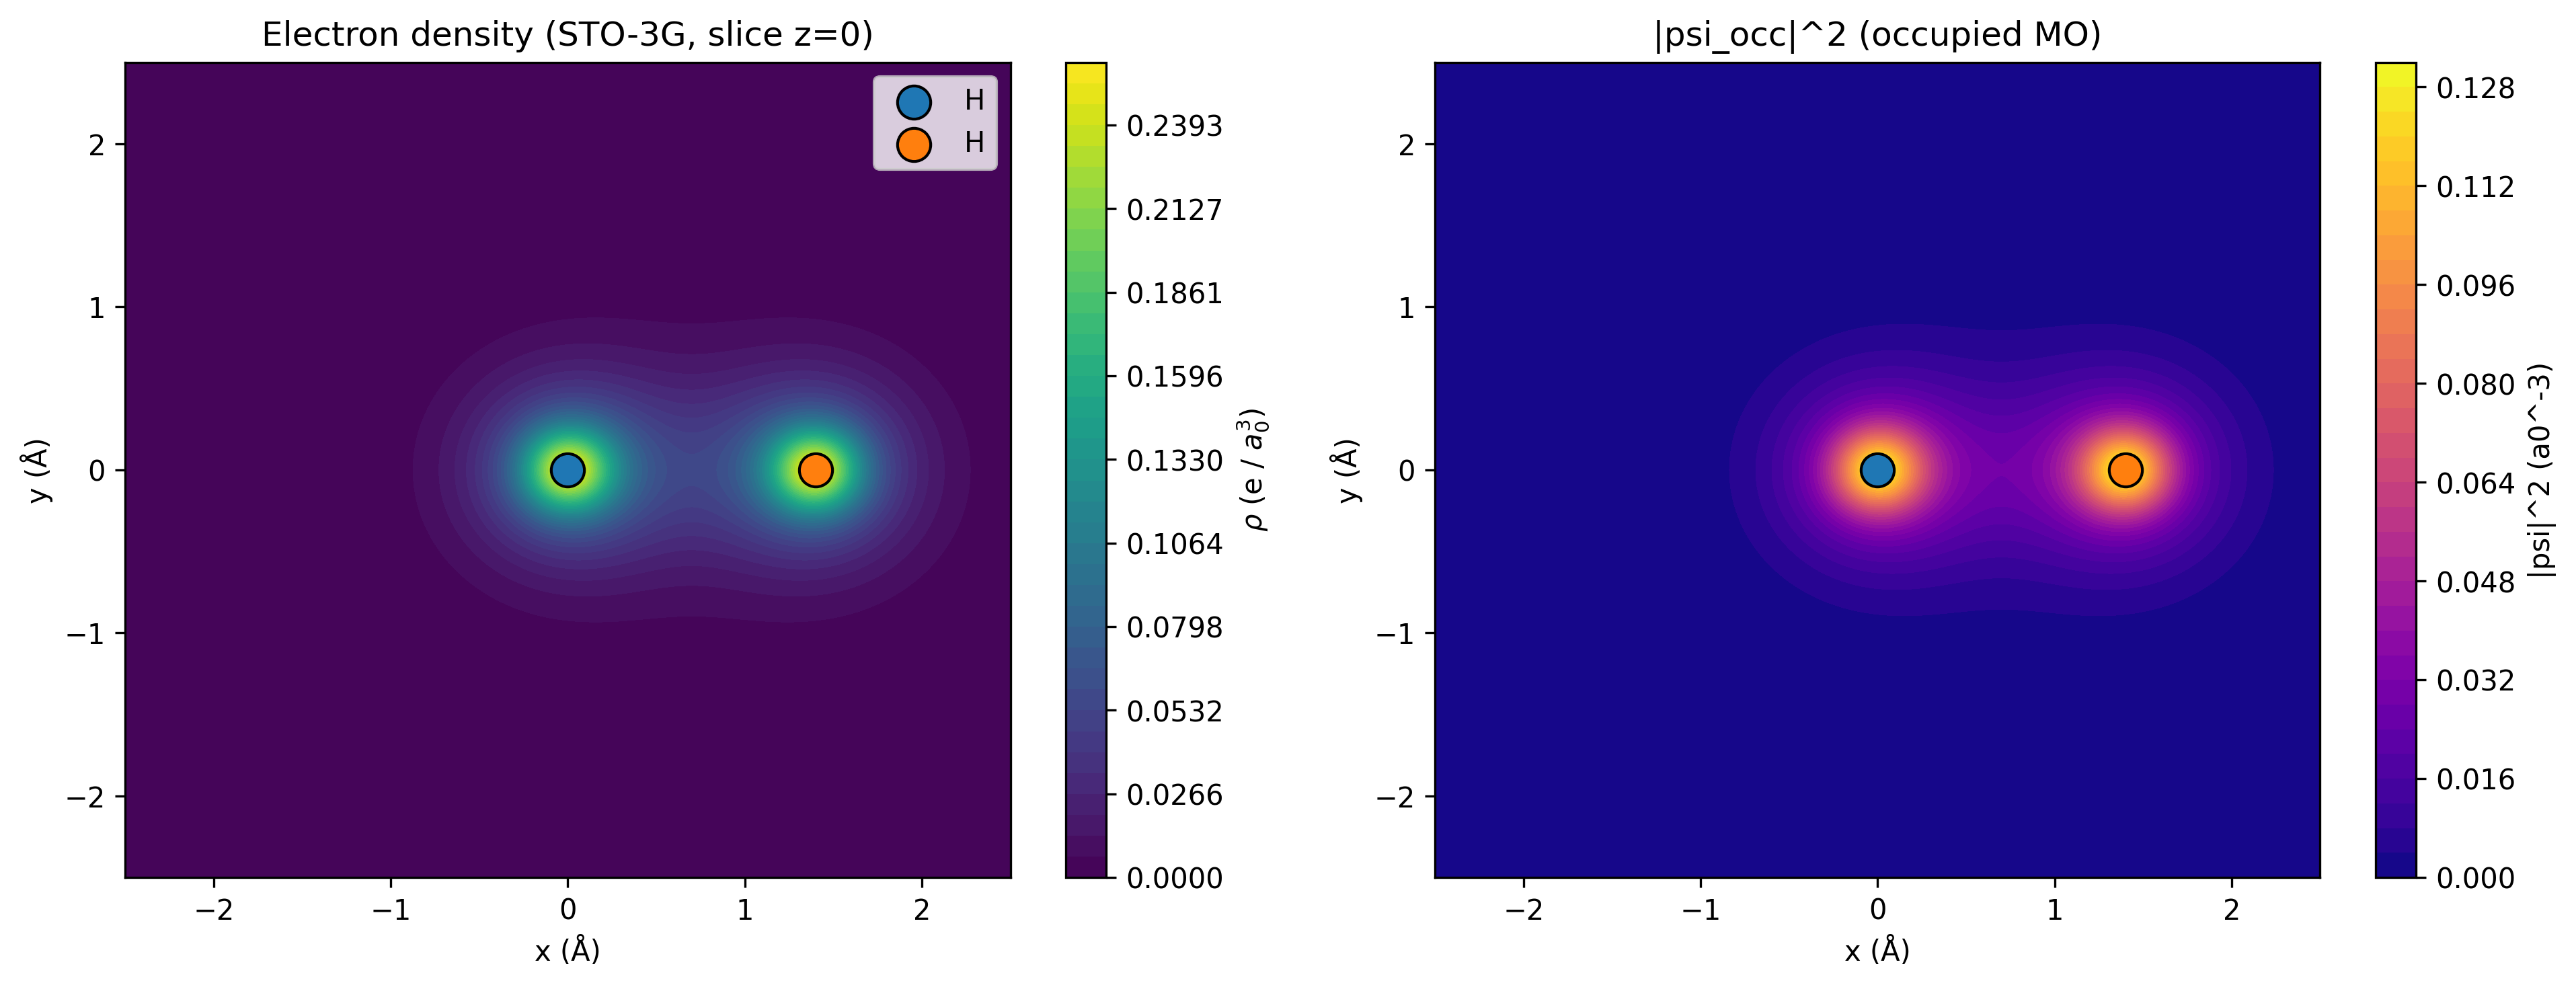
\includegraphics[width=0.95\linewidth]{density.png}\\[-0.2em]
{\small Densidad electrónica RHF (plano $z=0$).}\\[0.6em]
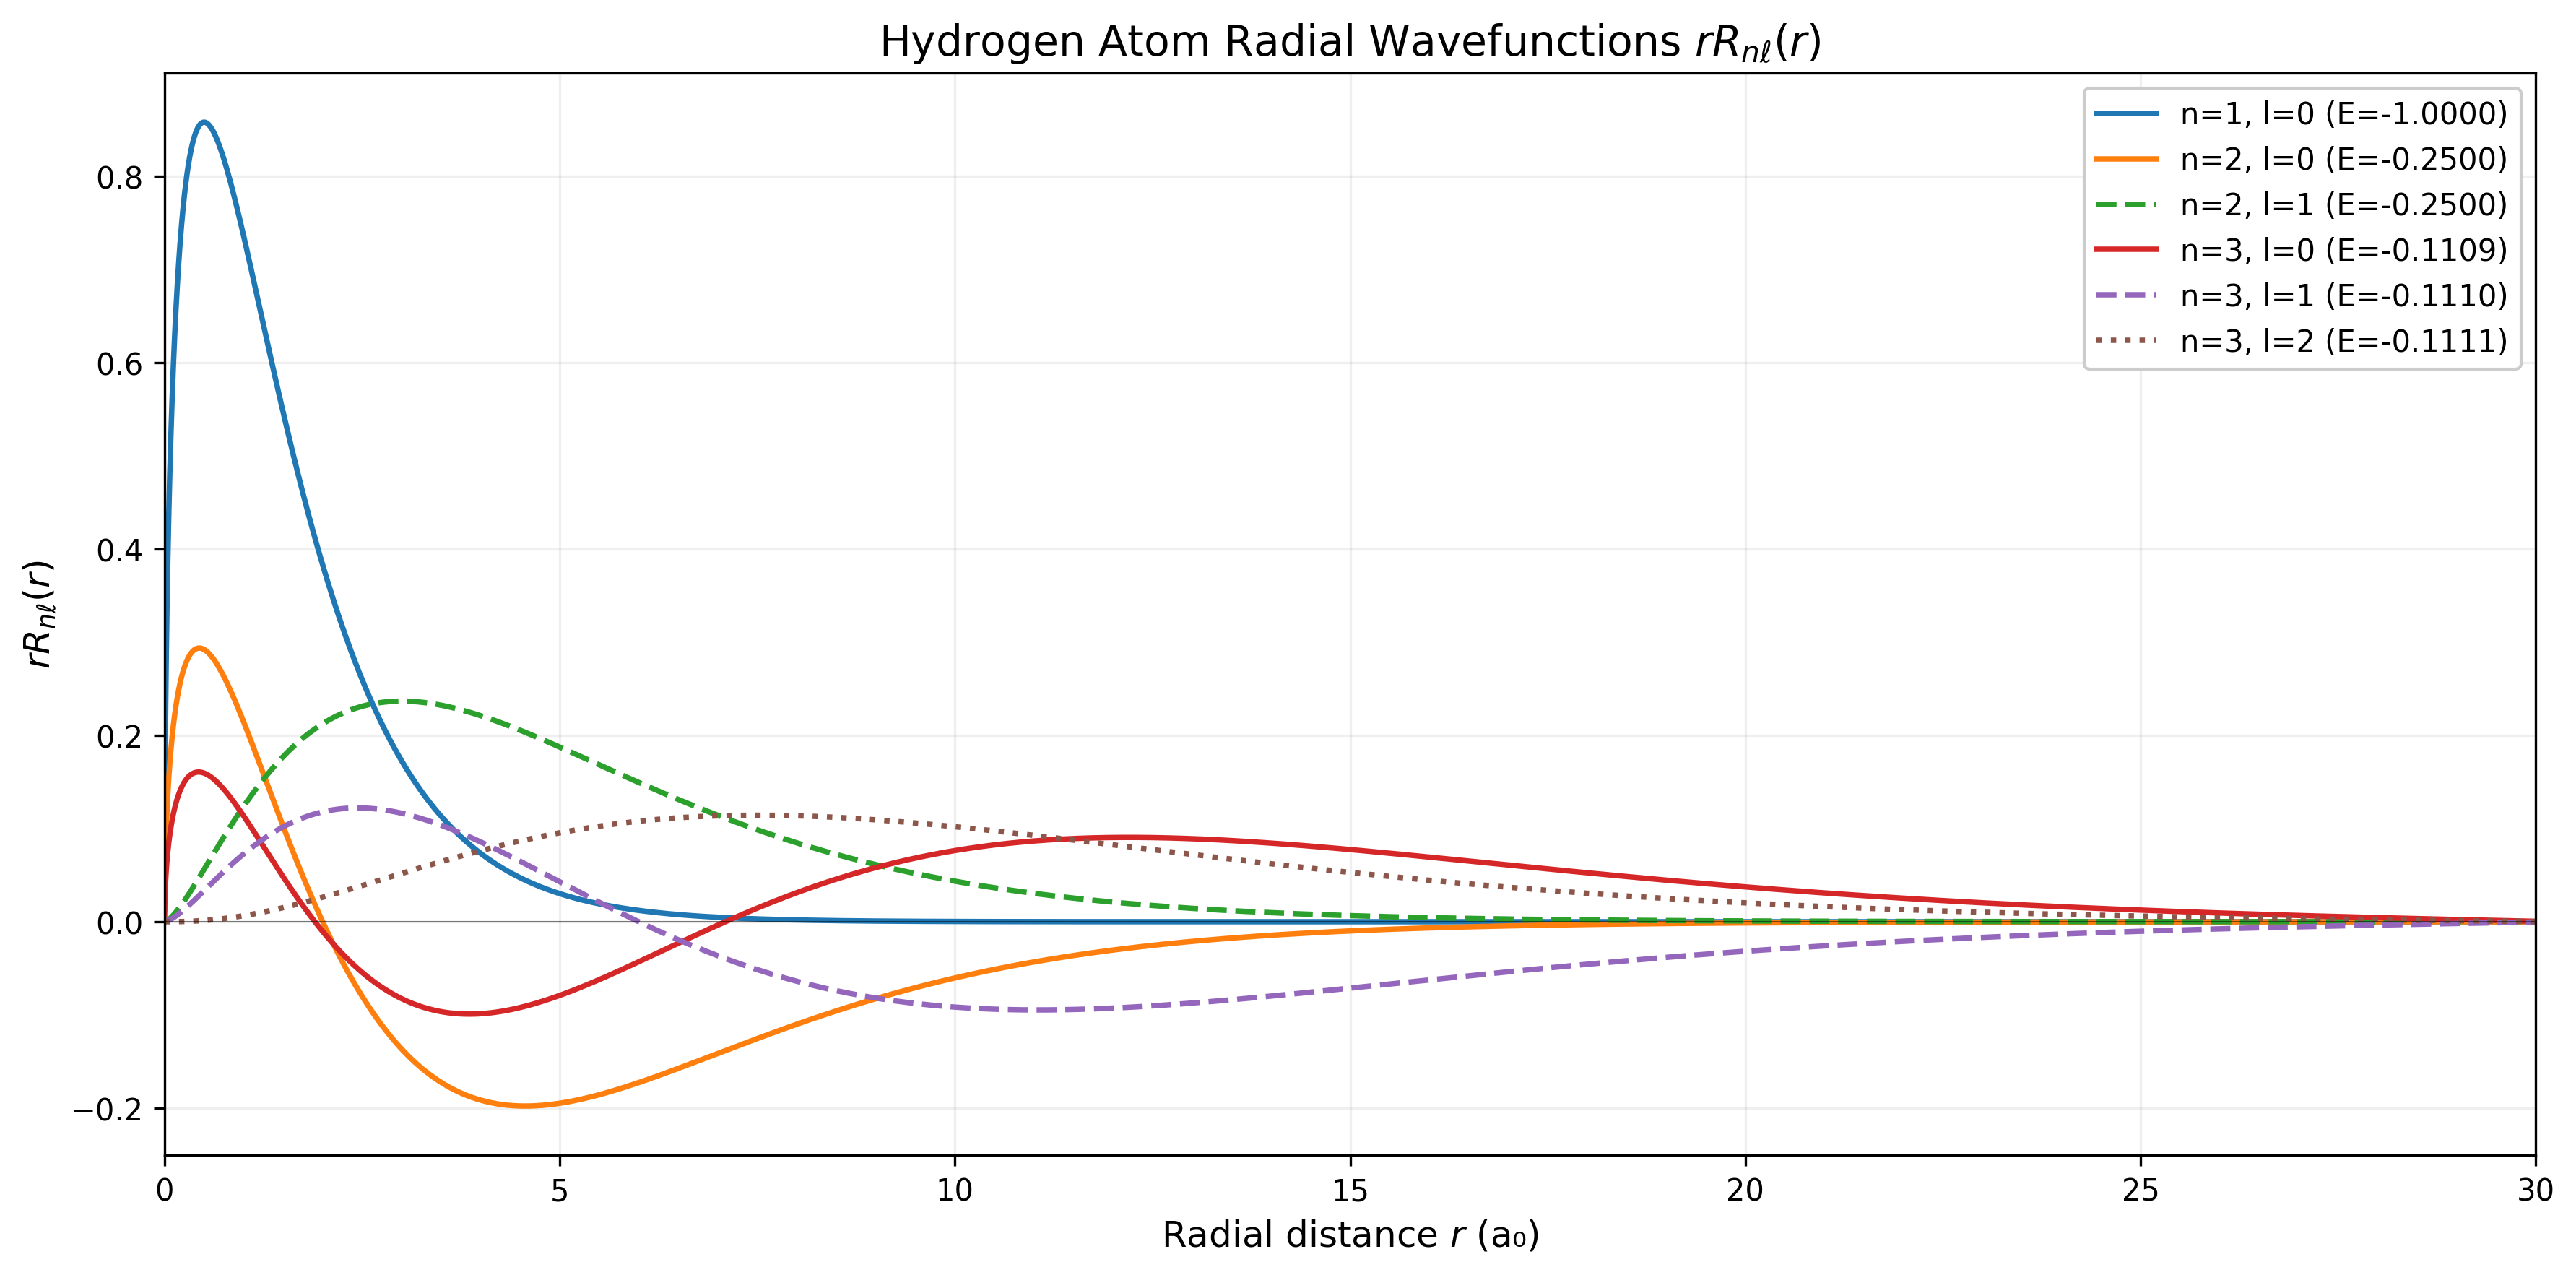
\includegraphics[width=0.95\linewidth]{hydrogen.png}\\[-0.2em]
{\small Curva $E_{\mathrm{tot}}(R)$ para H$_2$ (HF).}\\[0.6em]
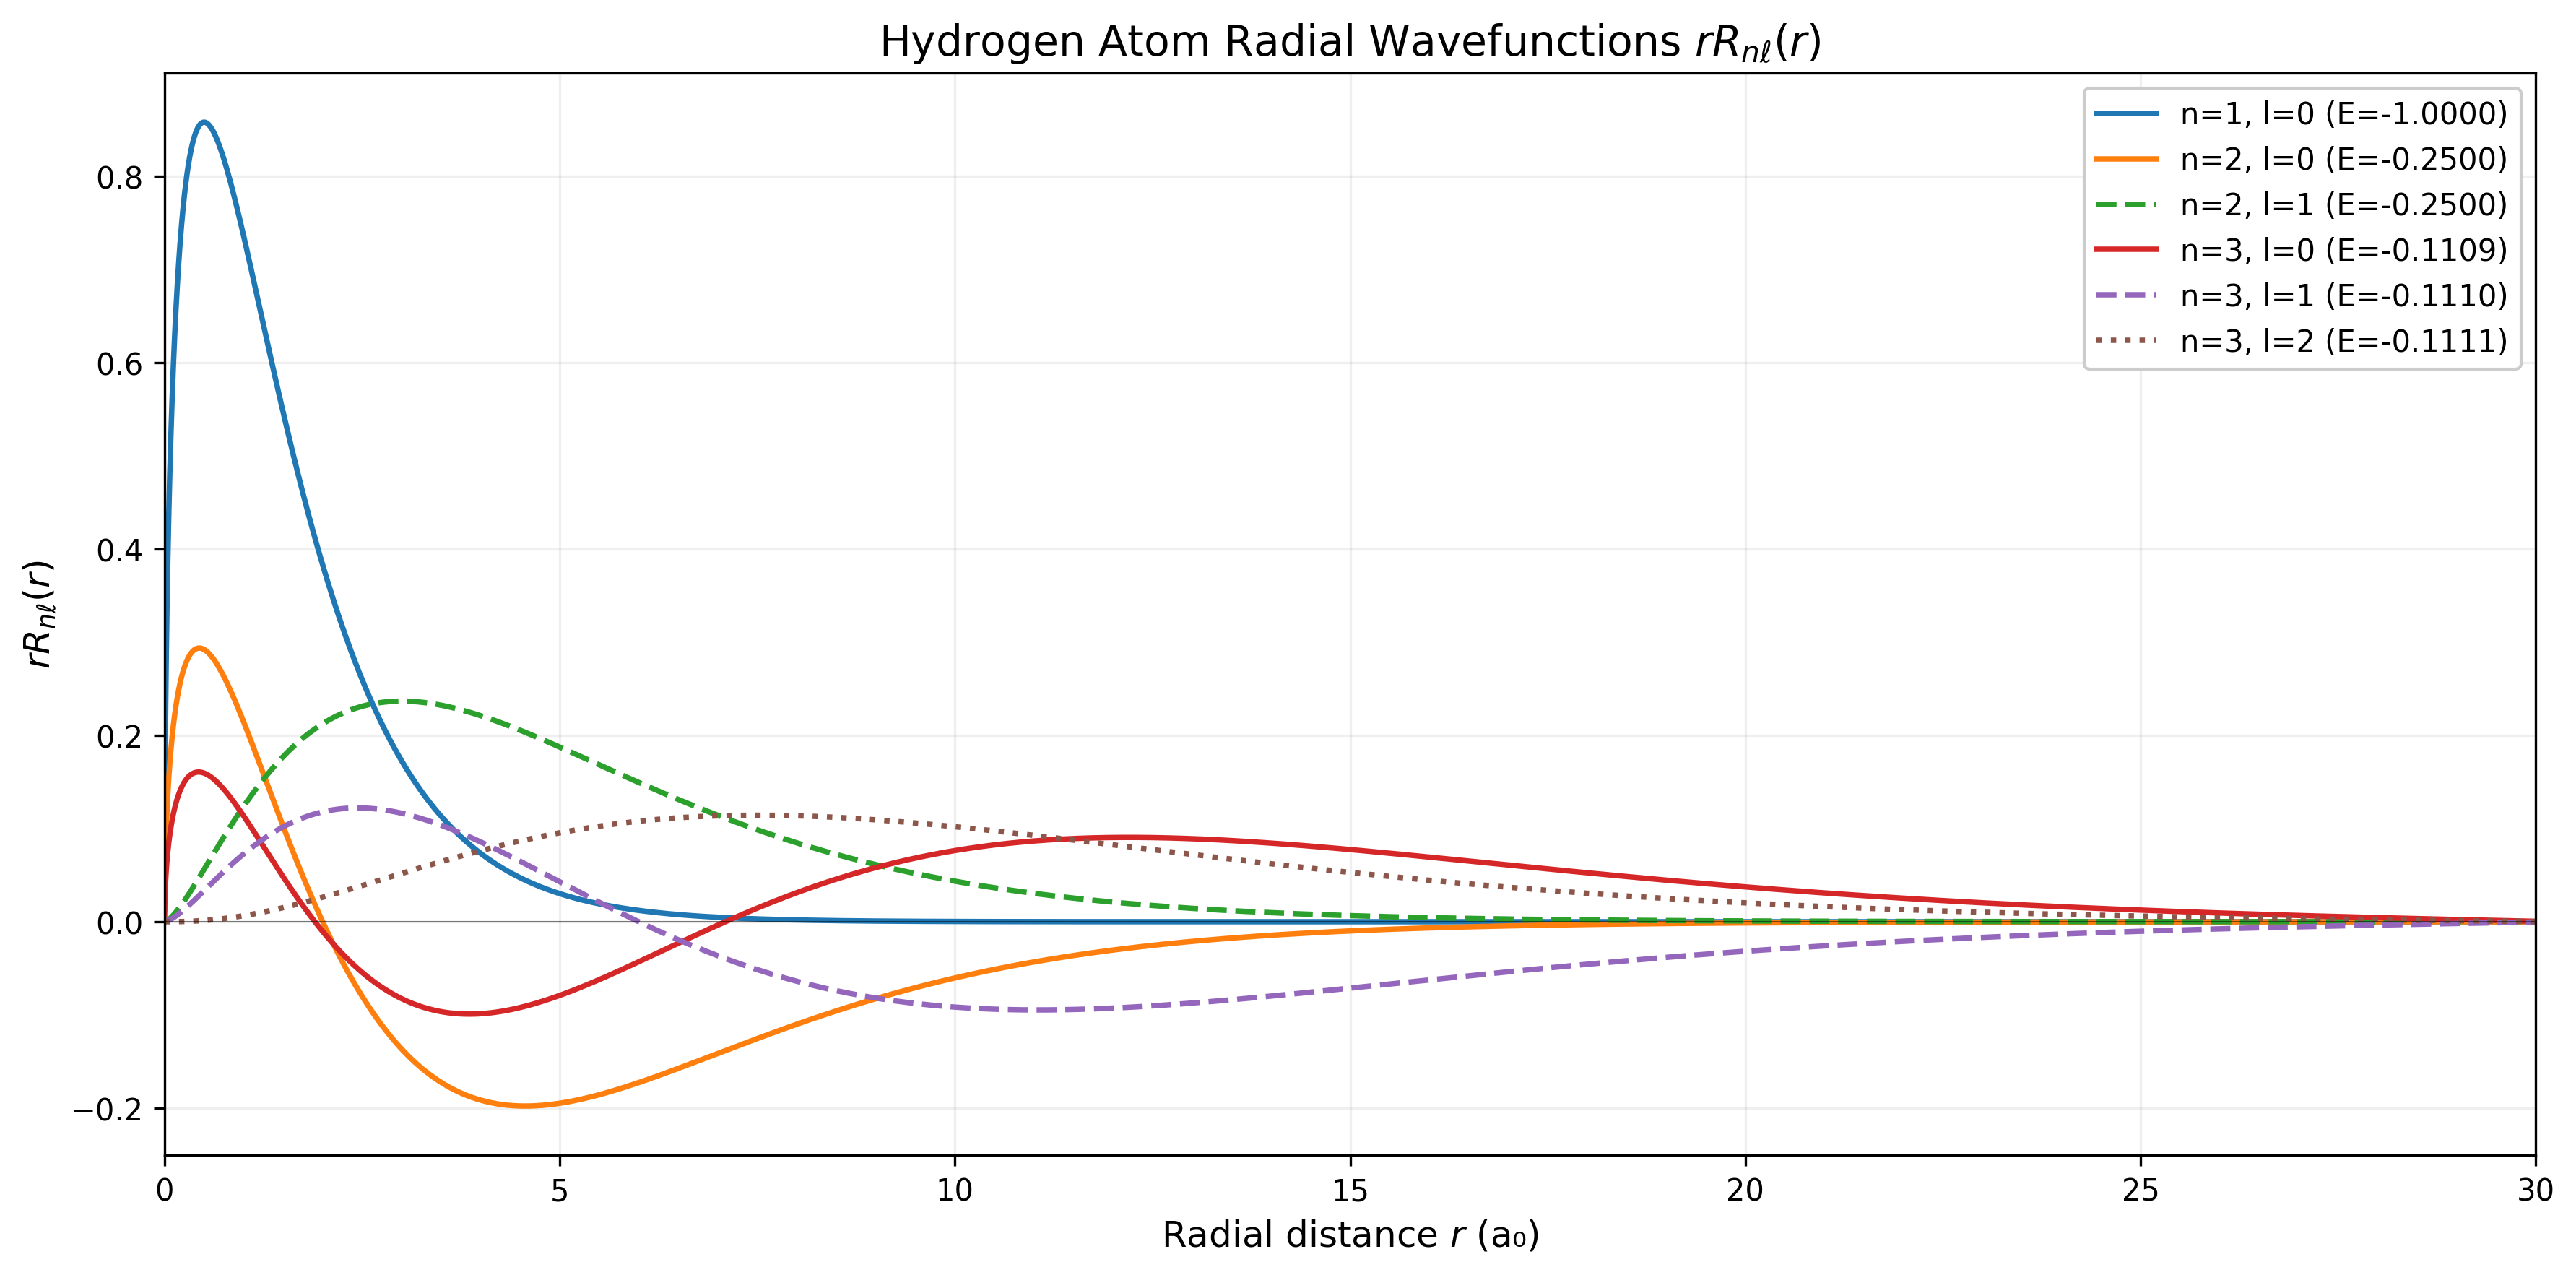
\includegraphics[width=0.95\linewidth]{hydrogen.png}\\[-0.2em]
{\small Curva $E_{\mathrm{tot}}(R)$ para HeH$^+$ (HF).}
\end{center}
\end{block}

\end{column}

% ===========================================================
% COLUMNA 3 — EXTRAS HF/PY + CONCLUSIONES + QR
% ===========================================================
\begin{column}{0.32\textwidth}

\begin{block}{Extensiones útiles (HF/Python)}
\textbf{Mulliken (cargas y orden de enlace)}:
\[
  G_A = \sum_{\mu\in A}\sum_\nu P_{\mu\nu} S_{\nu\mu},\quad
  q_A = Z_A - G_A,\quad
  BO_{AB}=\sum_{\mu\in A}\sum_{\nu\in B} P_{\mu\nu} S_{\nu\mu}.
\]
\textbf{Brecha HOMO--LUMO vs.\ $R$}: estabilidad y carácter del enlace.
\medskip

\textbf{Estrategia de código (repo)}:
\begin{itemize}
  \item \texttt{src/numerov/}: integrador y scripts OA/H.
  \item \texttt{src/hf/}: SCF (RHF), helpers de grilla para MO/densidad.
  \item \texttt{examples/}: \emph{PEC H$_2$}, \emph{PEC HeH$^+$}, \emph{MO maps}, \emph{Mulliken}.
  \item \texttt{docs/} (GitHub Pages): animaciones y derivaciones completas.
\end{itemize}

\textbf{Notas prácticas}:
\begin{itemize}
  \item Base mínima s-GTO \(\Rightarrow\) visualización rápida de $\sigma_g$, $\sigma_u$.
  \item Densidad en cortes 2D para el póster; 3D/isosuperficies en la web.
\end{itemize}
\end{block}

\begin{block}{Conclusiones}
\begin{itemize}
  \item Numerov y RHF acercan la MQ computacional al aula: \textbf{reproducible y extensible}.
  \item Las implementaciones en Python permiten conectar teoría, cómputo y visualización.
  \item El sitio web (QR) ofrece derivaciones completas y animaciones adicionales.
\end{itemize}
\end{block}

\begin{block}{Código y material extendido}
\begin{center}
\qrcode{https://github.com/recore799/schrodinger1d}\\[0.4em]
{\small \texttt{https://github.com/recore799/schrodinger1d}}
\end{center}
\end{block}

\end{column}

\end{columns}
\end{frame}
\end{document}
